\subsection{Quantization error}
In our coding, we use functions in the numpy library in python that will entail quantization error like np.where(). When calculating rise time, the 10\% and 90\% peak maximum is always underestimating the rise time a little because we use an inclusion condition to get the risetime interval. As the rising process is approximately linear, We have 4096 bins for the raw signal, assume the rising part takes k bins, the maximum quantization error is $\frac{2}{k}$ for the particular signal.

\subsection{Electronic Noise}
We notice that in Figure ref{1040} Nearly all of the low-energy part of the spectrum is eliminated through the use of event-selection filter. However, it might be the result of my method of calculating risetime, if the low-energy turns out to be like Figure. ref{example}, some electronic noise shots in the baseline even shoots higher than 10\% of the peak height will result in my counts of part smaller than 10\% peak height less than it should, thus overestimate the rise time a lot, which is reflected in the rise time histogram Figure. ref{old} where some unreasonably high rise time appears. To solve this problem, we change the code to ignore the baseline part and only focus on the rising part of the signal. We corrected the code and put the new result into the result section and the old ones in the appendix.
\begin{figure}[h!]
\begin{center}
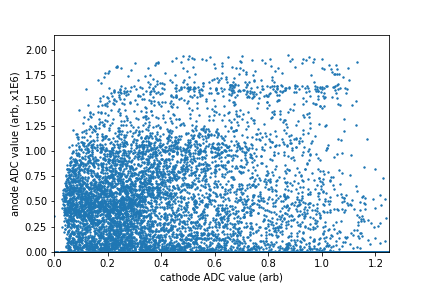
\includegraphics[scale=0.5]{scatter.png}
\caption{An example of a signal with poor SNR that result in bad calculation of rise time}
\label{example}
\end{center}
\end{figure}

\subsection{Pulse shape prediction}
The use of constant carrier drift velocity is convenient but also will induce error to our prediction. As for coaxial geometry, the irregularly increasing electric field will affect the velocity. However, we did not figure out a way to solve the loop interdependence of the three parameters.\\

Although the prediction for n-type detector accords with what is in the textbook, we have not compare the prediction of p-type signal to our set of signals. Ideally, we can find signals that look exactly like our prediction and count the numbers of each type and see if it corresponds with the coaxial geometry probablity of interaction position. 

\subsection{Conclusion}
The rise time discrimination points out that limiting the rise time to a optimal range will largely suppress noises, while degrade SNR by decreasing counts in the photopeak. The pulse shape prediction is given for both n-type and p-type HPGe detector, which accords with theoretical result.
\clearpage
\subsection*{Appendix}
\begin{figure}[h!]
\begin{center}
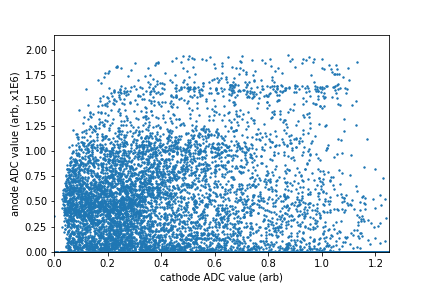
\includegraphics[scale=0.5]{scatter.png}
\caption{Old Rise time histogram}
\label{old}
\end{center}
\end{figure}
\begin{figure}[h!]
\begin{center}
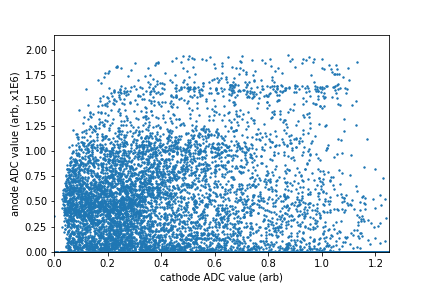
\includegraphics[scale=0.5]{scatter.png}
\caption{Old Original Spectrum}

\end{center}
\end{figure}
\begin{figure}[h!]
\begin{center}
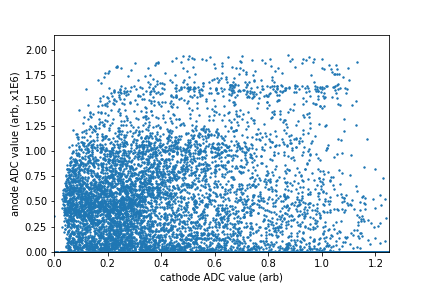
\includegraphics[scale=0.5]{scatter.png}
\caption{Old Spectrum of pulses with risetime between 100ns and 400ns}

\end{center}
\end{figure}

\begin{figure}[h!]
\begin{center}
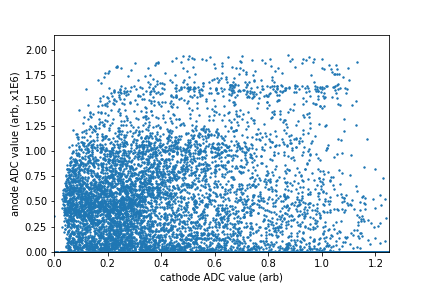
\includegraphics[scale=0.5]{scatter.png}
\caption{Old Spectrum of pulses with risetime between 400ns and 1000ns}
\end{center}
\end{figure}
\clearpage
\begin{table}[h!]
\begin{center}
\caption{Old PC and PT ratio for three spectrums}
\begin{tabular}{| c | c | c | c |}
\hline

	&\textbf{Original spectrum}  & \textbf{Ristime 100-400ns} & \textbf{Ristime 400-1000ns}\\\hline
	
PT ratio  	&0.1587		&0.2275		&0.001244 \\\hline

PC ratio	&0.2154		&0.3665		&0.001248 \\\hline

\end{tabular}

\end{center}
\end{table}
